\section{Model accuracy}

  \subsection{Cross validation}
    One of the main reasons for using cross-validation instead of using the conventional validation (e.g. partitioning the data set into two sets of 70\% for training and 30\% for test) is that there is not enough data available to partition it into separate training and test sets without losing significant modelling or testing capability. In these cases, a fair way to properly estimate model prediction performance is to use cross-validation as a powerful general technique. In summary, cross-validation combines (averages) measures of fit (prediction error) to derive a more accurate estimate of model prediction performance.
    \begin{figure}[htbp]
      \hspace*{-2cm}
      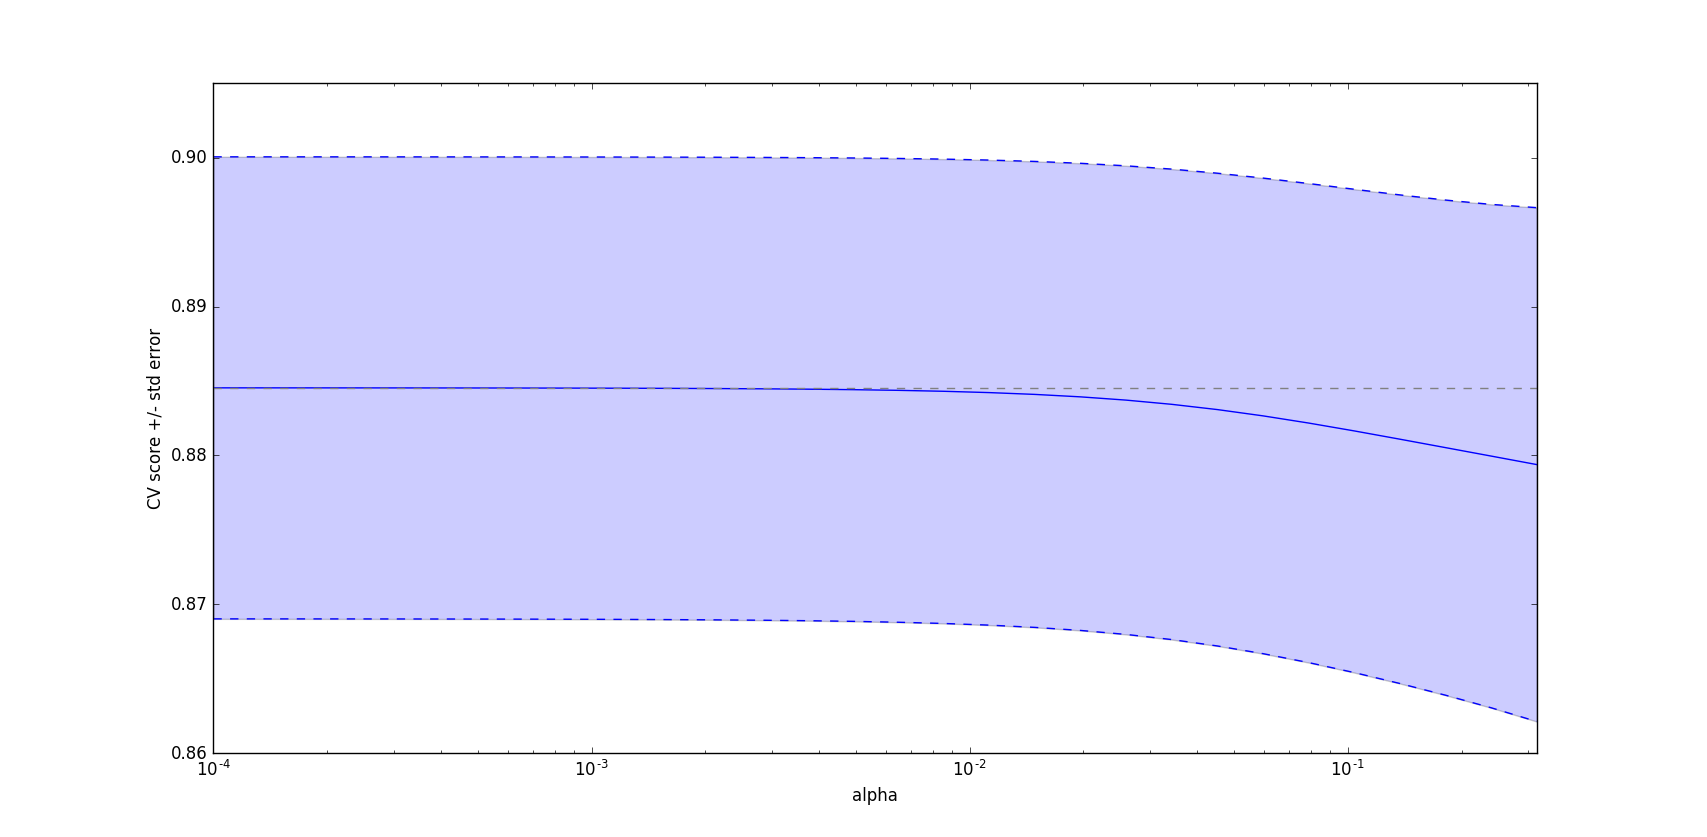
\includegraphics[width=1.2\linewidth]{cv.png}
      \caption{Cross-validation score for Ridge regression}
      \label{fig:cv}                    
    \end{figure}
\newpage
  \subsection{Linear vs Non-linear model}
  As observed before, the data has non-linear relationship with responses. The probability distributions demonstrate that none of the variables follows the normal distribution. Furthermore, the scatter plots show that any functional relationship of the input variables and the output variables is not trivial. This suggests that we can reasonably expect that classical learners such as linear regression (linear models) may fail to find an accurate mapping of the input variables to the output variables. Therefore, these insights intuitively show the need for non-linear models. This claim can be justified by comparing the accuracy of a linear model (Ridge regression) and non-linear model (ANN) below:
  \begin{figure}[h!]
      \centering
      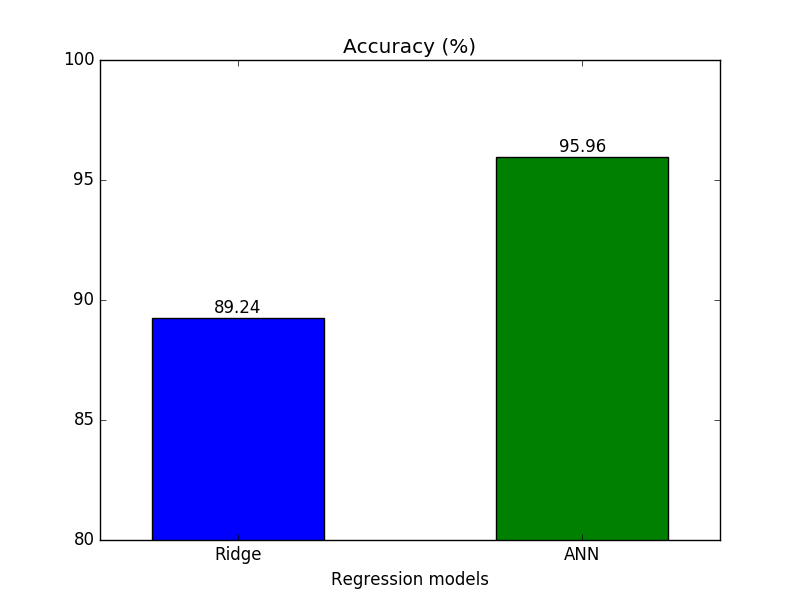
\includegraphics[width=0.9\linewidth]{accuracy.png}
      \caption{Models accuracy : Linear (Ridge) vs Non-linear (ANN)}
      \label{fig:accuracy}                    
  \end{figure}

